%%=============================================================================
%% LaTeX sjabloon voor bachelorproef, HoGent Bedrijf en Organisatie
%% Opleiding Toegepaste Informatica
%%=============================================================================

\documentclass[fleqn,a4paper,12pt]{book}

%%=============================================================================
%% LaTeX sjabloon voor de bachelorproef, HoGent Bedrijf en Organisatie
%% Opleiding toegepaste informatica
%%
%% Structuur en algemene vormgeving. Meestal hoef je hier niets te wijzigen.
%%
%% Vormgeving gebaseerd op "The Legrand Orange Book", version 2.0 (9/2/15)
%% door Mathias Legrand (legrand.mathias@gmail.com) met aanpassingen door
%% Vel (vel@latextemplates.com). Het oorspronkelijke template is te vinden op
%% http://www.LaTeXTemplates.com
%%
%% Aanpassingen voor HoGent toegepaste informatica: 
%%   Bert Van Vreckem <bert.vanvreckem@hogent.be>
%% Licentie: 
%%   CC BY-NC-SA 3.0 (http://creativecommons.org/licenses/by-nc-sa/3.0/)
%%=============================================================================

%%-----------------------------------------------------------------------------
%% Packages
%%-----------------------------------------------------------------------------

\usepackage[top=3cm,bottom=3cm,left=3cm,right=3cm,headsep=10pt,a4paper]{geometry} % Page margins
\usepackage[utf8]{inputenc}  % Accenten gebruiken in tekst (vb. é ipv \'e)
\usepackage{amsfonts}        % AMS math packages: extra wiskundige
\usepackage{amsmath}         %   symbolen (o.a. getallen-
\usepackage{amssymb}         %   verzamelingen N, R, Z, Q, etc.)
\usepackage[english,dutch]{babel}    % Taalinstellingen: woordsplitsingen,
                             %  commando's voor speciale karakters
                             %  ("dutch" voor NL)
\usepackage{iflang}
\usepackage{eurosym}         % Euro-symbool €
\usepackage{geometry}
\usepackage{graphicx}        % Invoegen van tekeningen
\graphicspath{{img/}}       % Specifies the directory where pictures are stored
\usepackage{tikz}            % Required for drawing custom shapes
\usepackage[pdftex,bookmarks=true]{hyperref}
                             % PDF krijgt klikbare links & verwijzingen,
                             %  inhoudstafel
\usepackage{enumitem}        % Customize lists
\setlist{nolistsep}         % Reduce spacing between list items
\usepackage{listings}        % Broncode mooi opmaken
\usepackage{multirow}        % Tekst over verschillende cellen in tabellen
\usepackage{rotating}        % Tabellen en figuren roteren

\usepackage{booktabs}        % Required for nicer horizontal rules in tables

\usepackage{xcolor}          % Required for specifying colors by name
\definecolor{maincolor}{RGB}{0,147,208} % Define the main color used for 
                             % highlighting throughout the book
                             % 0, 147, 208 = officiële kleur HoGent FBO

% Paragraph style: no indent, add space between paragraphs
\setlength{\parindent}{0em}
\setlength{\parskip}{1em}

\usepackage{etoolbox}
\usepackage{titling} % Macros for title, author, etc
\usepackage{lipsum}          % Voor vultekst (lorem ipsum)

%----------------------------------------------------------------------------------------
%	FONTS
%----------------------------------------------------------------------------------------

\usepackage{avant} % Use the Avantgarde font for headings
%\usepackage{times} % Use the Times font for headings
\usepackage{mathptmx} % Use the Adobe Times Roman as the default text font together with math symbols from the Sym­bol, Chancery and Com­puter Modern fonts

\usepackage{microtype} % Slightly tweak font spacing for aesthetics
\usepackage[utf8]{inputenc} % Required for including letters with accents
\usepackage[T1]{fontenc} % Use 8-bit encoding that has 256 glyphs

%------------------------------------------------------------------------------
%	TITLE PAGE
%------------------------------------------------------------------------------

\newcommand{\inserttitlepage}{%
\begin{titlepage}
  \newgeometry{top=2cm,bottom=1.5cm,left=1.5cm,right=1.5cm}
  \begin{center}

    \begingroup
    \rmfamily
    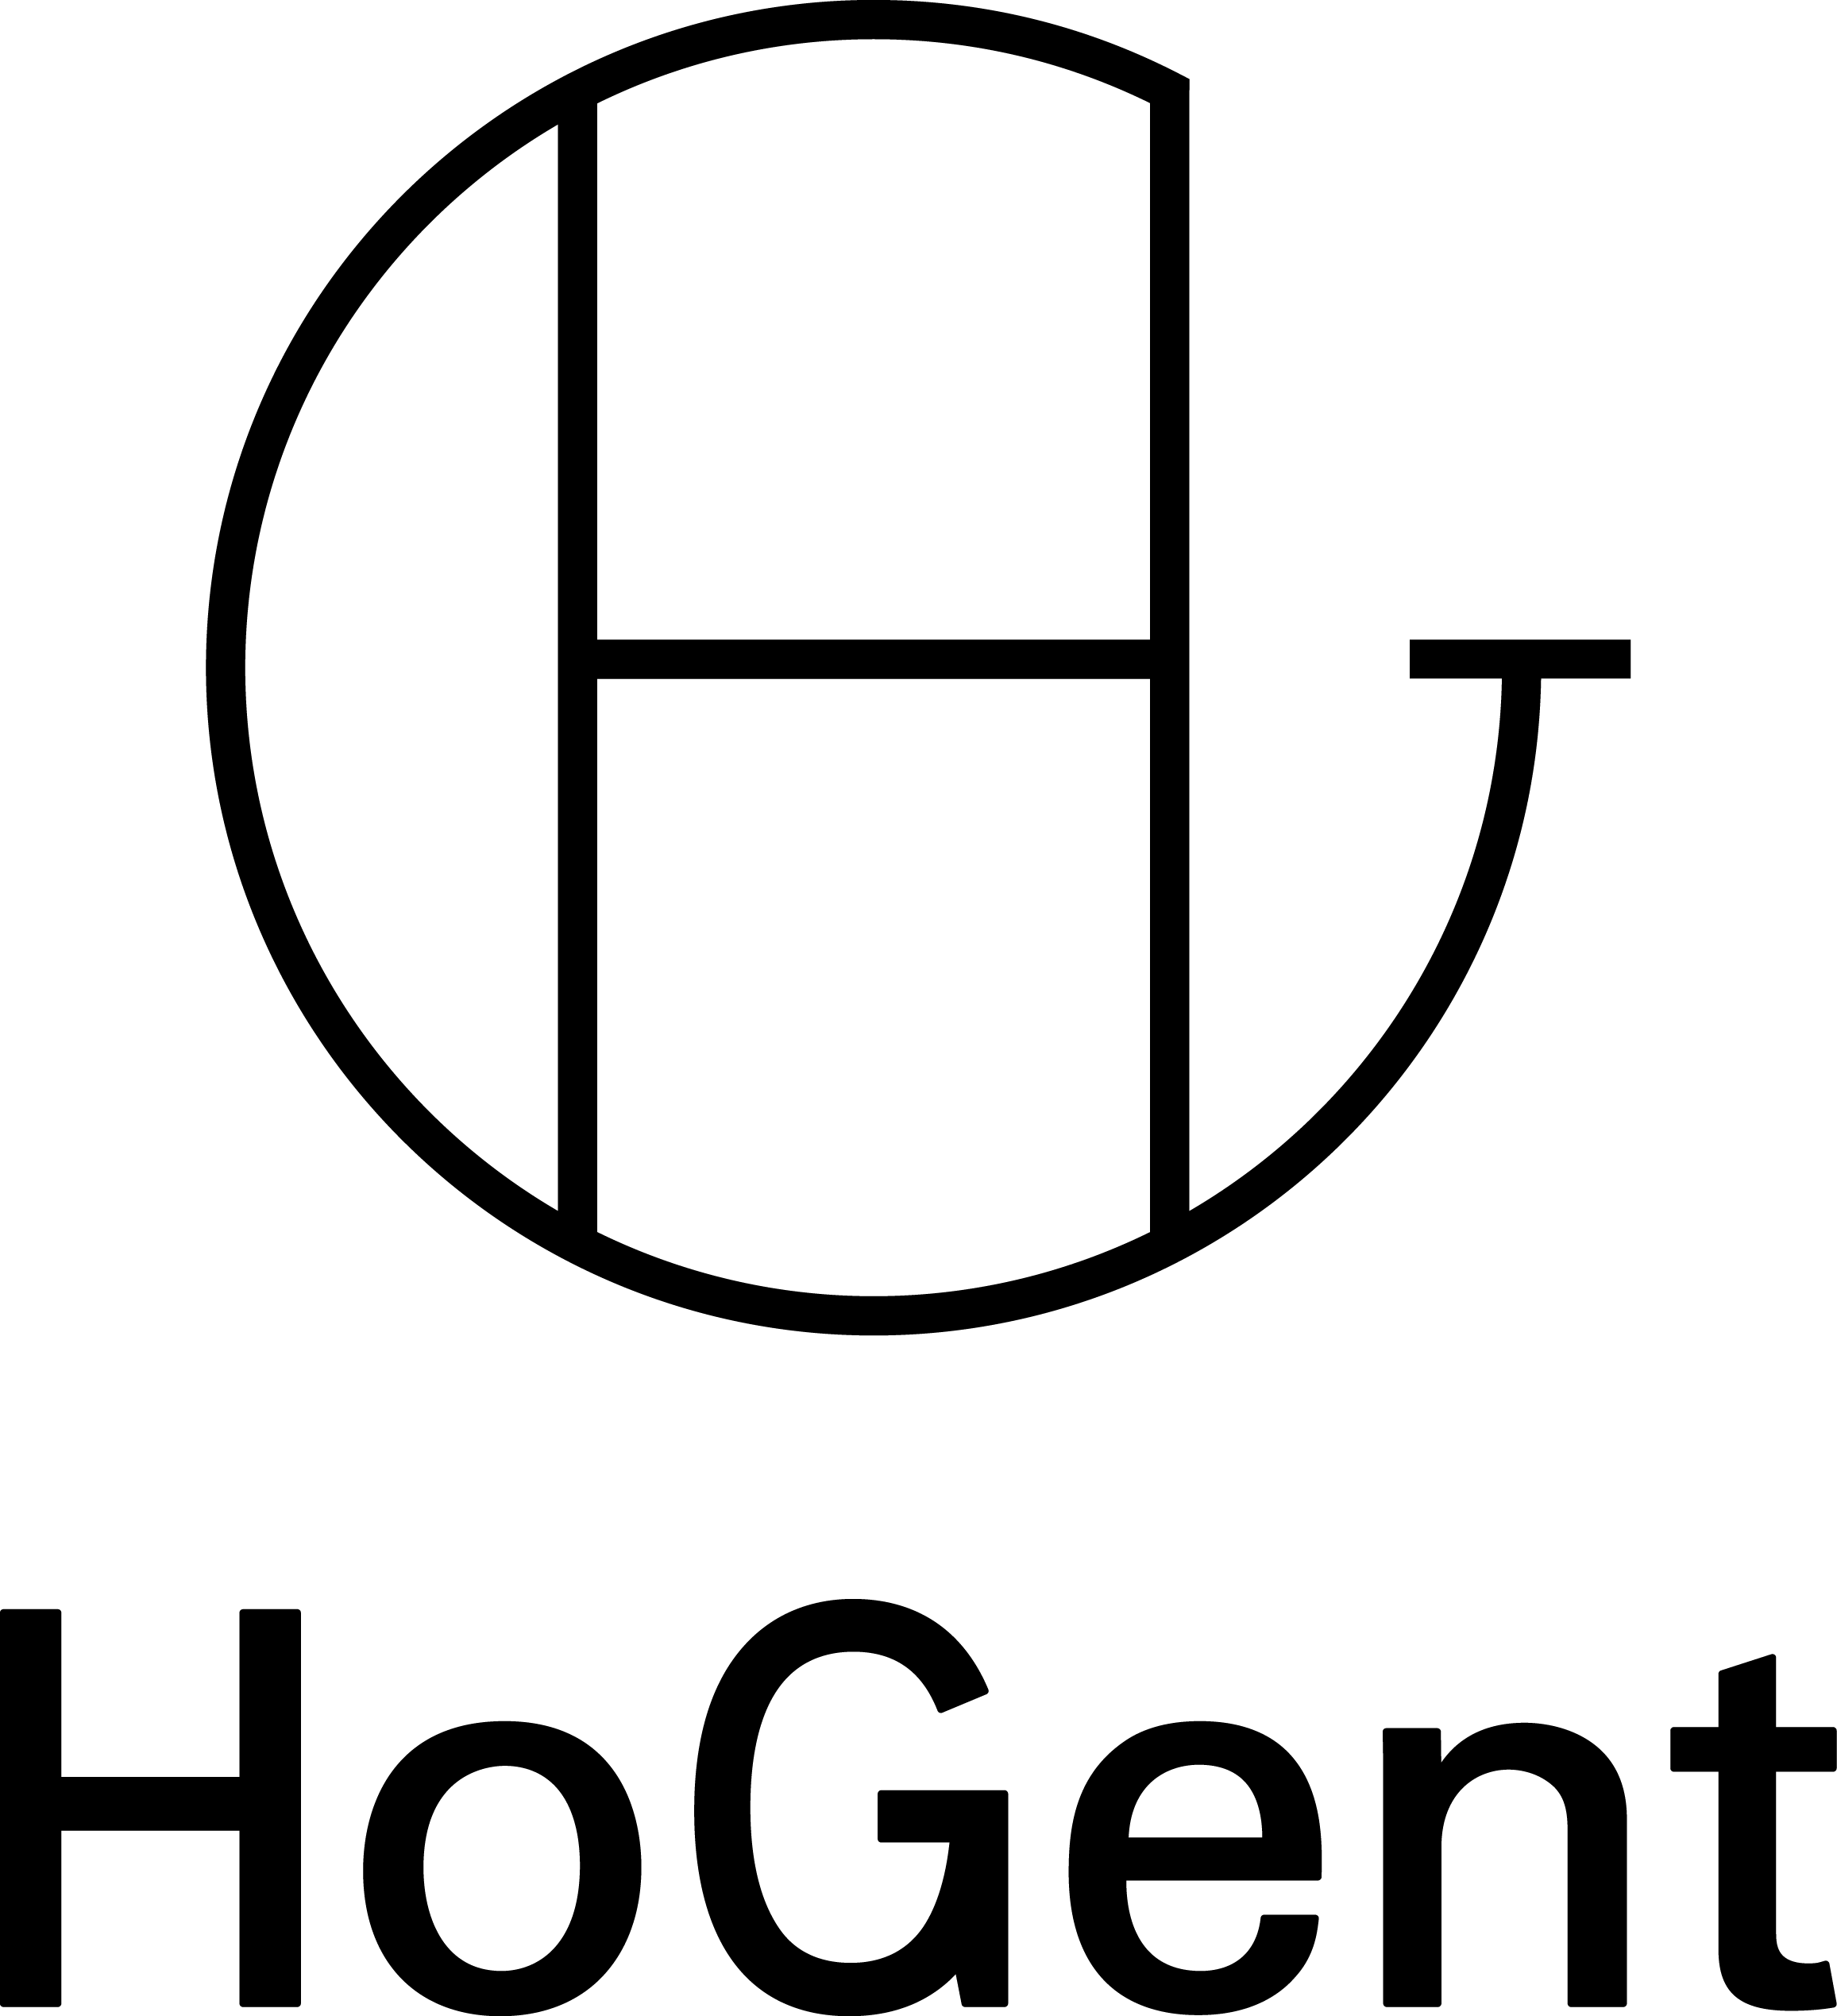
\includegraphics[width=2.5cm]{img/HG-beeldmerk-woordmerk}\\[.5cm]
    Faculteit Bedrijf en Organisatie\\[3cm]
    \titel
    \vfill
    \student\\[3.5cm]
    Scriptie voorgedragen tot het bekomen van de graad van\\professionele bachelor in de toegepaste informatica\\[2cm]
    Promotor:\\
    \promotor\\
    \ifdefempty{\copromotor}{\vspace{2.5cm}}{Co-promotor:\\\copromotor\\[2.5cm]}
    Instelling: \instelling\\[.5cm]
    Academiejaar: \academiejaar\\[.5cm]
    \ifcase \examenperiode \or Eerste \or Tweede \else Derde \fi examenperiode
    \endgroup

  \end{center}
  \restoregeometry
\end{titlepage}
  \emptypage
\begin{titlepage}
  \newgeometry{top=5.35cm,bottom=1.5cm,left=1.5cm,right=1.5cm}
  \begin{center}

    \begingroup
    \rmfamily
    \IfLanguageName{dutch}{Faculteit Bedrijf en Organisatie}{Faculty of Business and Information Management}\\[3cm]
    \titel
    \vfill
    \student\\[3.5cm]
    \IfLanguageName{dutch}{Scriptie voorgedragen tot het bekomen van de graad van\\professionele bachelor in de toegepaste informatica}{Thesis submitted in partial fulfilment of the requirements for the degree of\\professional bachelor of applied computer science}\\[2cm]
    Promotor:\\
    \promotor\\
    \ifdefempty{\copromotor}{\vspace{2.5cm}}{Co-promotor:\\\copromotor\\[2.5cm]}
    \IfLanguageName{dutch}{Instelling}{Institution}: \instelling\\[.5cm]
    \IfLanguageName{dutch}{Academiejaar}{Academic year}: \academiejaar\\[.5cm]
    \IfLanguageName{dutch}{%
    \ifcase \examenperiode \or Eerste \or Tweede \else Derde \fi examenperiode}{%
    \ifcase \examenperiode \or First \or Second \else Third \fi examination period}
    \endgroup

  \end{center}
  \restoregeometry
\end{titlepage}
}

%----------------------------------------------------------------------------------------
%	BIBLIOGRAPHY AND INDEX
%----------------------------------------------------------------------------------------

\usepackage[style=apa,backend=biber]{biblatex}
\usepackage{csquotes}
\DeclareLanguageMapping{dutch}{dutch-apa}
\addbibresource{bachproef-tin.bib} % BibTeX bibliography file
\addbibresource{../voorstel/voorstel.bib}
\defbibheading{bibempty}{}

\usepackage{calc} % For simpler calculation - used for spacing the index letter headings correctly
\usepackage{makeidx} % Required to make an index
\makeindex % Tells LaTeX to create the files required for indexing

%----------------------------------------------------------------------------------------
%	MAIN TABLE OF CONTENTS
%----------------------------------------------------------------------------------------

\usepackage{titletoc} % Required for manipulating the table of contents

\contentsmargin{0cm} % Removes the default margin

% Part text styling
\titlecontents{part}[0cm]
{\addvspace{20pt}\centering\large\bfseries}
{}
{}
{}

% Chapter text styling
\titlecontents{chapter}[1.25cm] % Indentation
{\addvspace{12pt}\large\sffamily\bfseries} % Spacing and font options for chapters
{\color{maincolor!60}\contentslabel[\Large\thecontentslabel]{1.25cm}\color{maincolor}} % Chapter number
{\color{maincolor}}
{\color{maincolor!60}\normalsize\;\titlerule*[.5pc]{.}\;\thecontentspage} % Page number

% Section text styling
\titlecontents{section}[1.25cm] % Indentation
{\addvspace{3pt}\sffamily\bfseries} % Spacing and font options for sections
{\contentslabel[\thecontentslabel]{1.25cm}} % Section number
{}
{\hfill\color{black}\thecontentspage} % Page number
[]

% Subsection text styling
\titlecontents{subsection}[1.25cm] % Indentation
{\addvspace{1pt}\sffamily\small} % Spacing and font options for subsections
{\contentslabel[\thecontentslabel]{1.25cm}} % Subsection number
{}
{\ \titlerule*[.5pc]{.}\;\thecontentspage} % Page number
[]

% List of figures
\titlecontents{figure}[0em]
{\addvspace{-5pt}\sffamily}
{\thecontentslabel\hspace*{1em}}
{}
{\ \titlerule*[.5pc]{.}\;\thecontentspage}
[]

% List of tables
\titlecontents{table}[0em]
{\addvspace{-5pt}\sffamily}
{\thecontentslabel\hspace*{1em}}
{}
{\ \titlerule*[.5pc]{.}\;\thecontentspage}
[]

%----------------------------------------------------------------------------------------
%	MINI TABLE OF CONTENTS IN PART HEADS
%----------------------------------------------------------------------------------------

% Chapter text styling
\titlecontents{lchapter}[0em] % Indenting
{\addvspace{15pt}\large\sffamily\bfseries} % Spacing and font options for chapters
{\color{maincolor}\contentslabel[\Large\thecontentslabel]{1.25cm}\color{maincolor}} % Chapter number
{}
{\color{maincolor}\normalsize\sffamily\bfseries\;\titlerule*[.5pc]{.}\;\thecontentspage} % Page number

% Section text styling
\titlecontents{lsection}[0em] % Indenting
{\sffamily\small} % Spacing and font options for sections
{\contentslabel[\thecontentslabel]{1.25cm}} % Section number
{}
{}

% Subsection text styling
\titlecontents{lsubsection}[.5em] % Indentation
{\normalfont\footnotesize\sffamily} % Font settings
{}
{}
{}

%----------------------------------------------------------------------------------------
%	PAGE HEADERS
%----------------------------------------------------------------------------------------

\usepackage{fancyhdr} % Required for header and footer configuration

\pagestyle{fancy}
\renewcommand{\chaptermark}[1]{\markboth{\sffamily\normalsize\bfseries\chaptername\ \thechapter.\ #1}{}} % Chapter text font settings
\renewcommand{\sectionmark}[1]{\markright{\sffamily\normalsize\thesection\hspace{5pt}#1}{}} % Section text font settings
\fancyhf{} \fancyhead[LE,RO]{\sffamily\normalsize\thepage} % Font setting for the page number in the header
\fancyhead[LO]{\rightmark} % Print the nearest section name on the left side of odd pages
\fancyhead[RE]{\leftmark} % Print the current chapter name on the right side of even pages
\renewcommand{\headrulewidth}{0.5pt} % Width of the rule under the header
\addtolength{\headheight}{2.5pt} % Increase the spacing around the header slightly
\renewcommand{\footrulewidth}{0pt} % Removes the rule in the footer
\fancypagestyle{plain}{\fancyhead{}\renewcommand{\headrulewidth}{0pt}} % Style for when a plain pagestyle is specified

% Removes the header from odd empty pages at the end of chapters
\makeatletter
\renewcommand{\cleardoublepage}{
\clearpage\ifodd\c@page\else
\hbox{}
\vspace*{\fill}
\thispagestyle{empty}
\newpage
\fi}

%----------------------------------------------------------------------------------------
%	THEOREM STYLES
%----------------------------------------------------------------------------------------

\usepackage{amsmath,amsfonts,amssymb,amsthm} % For math equations, theorems, symbols, etc

\newcommand{\intoo}[2]{\mathopen{]}#1\,;#2\mathclose{[}}
\newcommand{\ud}{\mathop{\mathrm{{}d}}\mathopen{}}
\newcommand{\intff}[2]{\mathopen{[}#1\,;#2\mathclose{]}}
\newtheorem{notation}{Notation}[chapter]

% Boxed/framed environments
\newtheoremstyle{maincolornumbox}% % Theorem style name
{0pt}% Space above
{0pt}% Space below
{\normalfont}% % Body font
{}% Indent amount
{\small\bf\sffamily\color{maincolor}}% % Theorem head font
{\;}% Punctuation after theorem head
{0.25em}% Space after theorem head
{\small\sffamily\color{maincolor}\thmname{#1}\nobreakspace\thmnumber{\@ifnotempty{#1}{}\@upn{#2}}% Theorem text (e.g. Theorem 2.1)
\thmnote{\nobreakspace\the\thm@notefont\sffamily\bfseries\color{black}---\nobreakspace#3.}} % Optional theorem note
\renewcommand{\qedsymbol}{$\blacksquare$}% Optional qed square

\newtheoremstyle{blacknumex}% Theorem style name
{5pt}% Space above
{5pt}% Space below
{\normalfont}% Body font
{} % Indent amount
{\small\bf\sffamily}% Theorem head font
{\;}% Punctuation after theorem head
{0.25em}% Space after theorem head
{\small\sffamily{\tiny\ensuremath{\blacksquare}}\nobreakspace\thmname{#1}\nobreakspace\thmnumber{\@ifnotempty{#1}{}\@upn{#2}}% Theorem text (e.g. Theorem 2.1)
\thmnote{\nobreakspace\the\thm@notefont\sffamily\bfseries---\nobreakspace#3.}}% Optional theorem note

\newtheoremstyle{blacknumbox} % Theorem style name
{0pt}% Space above
{0pt}% Space below
{\normalfont}% Body font
{}% Indent amount
{\small\bf\sffamily}% Theorem head font
{\;}% Punctuation after theorem head
{0.25em}% Space after theorem head
{\small\sffamily\thmname{#1}\nobreakspace\thmnumber{\@ifnotempty{#1}{}\@upn{#2}}% Theorem text (e.g. Theorem 2.1)
\thmnote{\nobreakspace\the\thm@notefont\sffamily\bfseries---\nobreakspace#3.}}% Optional theorem note

% Non-boxed/non-framed environments
\newtheoremstyle{maincolornum}% % Theorem style name
{5pt}% Space above
{5pt}% Space below
{\normalfont}% % Body font
{}% Indent amount
{\small\bf\sffamily\color{maincolor}}% % Theorem head font
{\;}% Punctuation after theorem head
{0.25em}% Space after theorem head
{\small\sffamily\color{maincolor}\thmname{#1}\nobreakspace\thmnumber{\@ifnotempty{#1}{}\@upn{#2}}% Theorem text (e.g. Theorem 2.1)
\thmnote{\nobreakspace\the\thm@notefont\sffamily\bfseries\color{black}---\nobreakspace#3.}} % Optional theorem note
\renewcommand{\qedsymbol}{$\blacksquare$}% Optional qed square
\makeatother

% Defines the theorem text style for each type of theorem to one of the three styles above
\newcounter{dummy}
\numberwithin{dummy}{section}
\theoremstyle{maincolornumbox}
\newtheorem{theoremeT}[dummy]{Theorem}
\newtheorem{problem}{Problem}[chapter]
\newtheorem{exerciseT}{Exercise}[chapter]
\theoremstyle{blacknumex}
\newtheorem{exampleT}{Example}[chapter]
\theoremstyle{blacknumbox}
\newtheorem{vocabulary}{Vocabulary}[chapter]
\newtheorem{definitionT}{Definition}[section]
\newtheorem{corollaryT}[dummy]{Corollary}
\theoremstyle{maincolornum}
\newtheorem{proposition}[dummy]{Proposition}

%----------------------------------------------------------------------------------------
%	DEFINITION OF COLORED BOXES
%----------------------------------------------------------------------------------------

\RequirePackage[framemethod=default]{mdframed} % Required for creating the theorem, definition, exercise and corollary boxes

% Theorem box
\newmdenv[skipabove=7pt,
skipbelow=7pt,
backgroundcolor=black!5,
linecolor=maincolor,
innerleftmargin=5pt,
innerrightmargin=5pt,
innertopmargin=5pt,
leftmargin=0cm,
rightmargin=0cm,
innerbottommargin=5pt]{tBox}

% Exercise box
\newmdenv[skipabove=7pt,
skipbelow=7pt,
rightline=false,
leftline=true,
topline=false,
bottomline=false,
backgroundcolor=maincolor!10,
linecolor=maincolor,
innerleftmargin=5pt,
innerrightmargin=5pt,
innertopmargin=5pt,
innerbottommargin=5pt,
leftmargin=0cm,
rightmargin=0cm,
linewidth=4pt]{eBox}

% Definition box
\newmdenv[skipabove=7pt,
skipbelow=7pt,
rightline=false,
leftline=true,
topline=false,
bottomline=false,
linecolor=maincolor,
innerleftmargin=5pt,
innerrightmargin=5pt,
innertopmargin=0pt,
leftmargin=0cm,
rightmargin=0cm,
linewidth=4pt,
innerbottommargin=0pt]{dBox}

% Corollary box
\newmdenv[skipabove=7pt,
skipbelow=7pt,
rightline=false,
leftline=true,
topline=false,
bottomline=false,
linecolor=gray,
backgroundcolor=black!5,
innerleftmargin=5pt,
innerrightmargin=5pt,
innertopmargin=5pt,
leftmargin=0cm,
rightmargin=0cm,
linewidth=4pt,
innerbottommargin=5pt]{cBox}

% Creates an environment for each type of theorem and assigns it a theorem text style from the "Theorem Styles" section above and a colored box from above
\newenvironment{theorem}{\begin{tBox}\begin{theoremeT}}{\end{theoremeT}\end{tBox}}
\newenvironment{exercise}{\begin{eBox}\begin{exerciseT}}{\hfill{\color{maincolor}\tiny\ensuremath{\blacksquare}}\end{exerciseT}\end{eBox}}
\newenvironment{definition}{\begin{dBox}\begin{definitionT}}{\end{definitionT}\end{dBox}}
\newenvironment{example}{\begin{exampleT}}{\hfill{\tiny\ensuremath{\blacksquare}}\end{exampleT}}
\newenvironment{corollary}{\begin{cBox}\begin{corollaryT}}{\end{corollaryT}\end{cBox}}

%----------------------------------------------------------------------------------------
%	REMARK ENVIRONMENT
%----------------------------------------------------------------------------------------

\newenvironment{remark}{\par\vspace{10pt}\small % Vertical white space above the remark and smaller font size
\begin{list}{}{
\leftmargin=35pt % Indentation on the left
\rightmargin=25pt}\item\ignorespaces % Indentation on the right
\makebox[-2.5pt]{\begin{tikzpicture}[overlay]
\node[draw=maincolor!60,line width=1pt,circle,fill=maincolor!25,font=\sffamily\bfseries,inner sep=2pt,outer sep=0pt] at (-15pt,0pt){\textcolor{maincolor}{R}};\end{tikzpicture}} % Orange R in a circle
\advance\baselineskip -1pt}{\end{list}\vskip5pt} % Tighter line spacing and white space after remark

%----------------------------------------------------------------------------------------
%	SECTION NUMBERING IN THE MARGIN
%----------------------------------------------------------------------------------------

\makeatletter
\renewcommand{\@seccntformat}[1]{\llap{\textcolor{maincolor}{\csname the#1\endcsname}\hspace{1em}}}
\renewcommand{\section}{\@startsection{section}{1}{\z@}
{-4ex \@plus -1ex \@minus -.4ex}
{1ex \@plus.2ex }
{\normalfont\large\sffamily\bfseries}}
\renewcommand{\subsection}{\@startsection {subsection}{2}{\z@}
{-3ex \@plus -0.1ex \@minus -.4ex}
{0.5ex \@plus.2ex }
{\normalfont\sffamily\bfseries}}
\renewcommand{\subsubsection}{\@startsection {subsubsection}{3}{\z@}
{-2ex \@plus -0.1ex \@minus -.2ex}
{.2ex \@plus.2ex }
{\normalfont\small\sffamily\bfseries}}
\renewcommand\paragraph{\@startsection{paragraph}{4}{\z@}
{-2ex \@plus-.2ex \@minus .2ex}
{.1ex}
{\normalfont\small\sffamily\bfseries}}

%----------------------------------------------------------------------------------------
%	PART HEADINGS
%----------------------------------------------------------------------------------------

% numbered part in the table of contents
\newcommand{\@mypartnumtocformat}[2]{%
\setlength\fboxsep{0pt}%
\noindent\colorbox{maincolor!20}{\strut\parbox[c][.7cm]{\ecart}{\color{maincolor!70}\Large\sffamily\bfseries\centering#1}}\hskip\esp\colorbox{maincolor!40}{\strut\parbox[c][.7cm]{\linewidth-\ecart-\esp}{\Large\sffamily\centering#2}}}%
%%%%%%%%%%%%%%%%%%%%%%%%%%%%%%%%%%
% unnumbered part in the table of contents
\newcommand{\@myparttocformat}[1]{%
\setlength\fboxsep{0pt}%
\noindent\colorbox{maincolor!40}{\strut\parbox[c][.7cm]{\linewidth}{\Large\sffamily\centering#1}}}%
%%%%%%%%%%%%%%%%%%%%%%%%%%%%%%%%%%
\newlength\esp
\setlength\esp{4pt}
\newlength\ecart
\setlength\ecart{1.2cm-\esp}
\newcommand{\thepartimage}{}%
\newcommand{\partimage}[1]{\renewcommand{\thepartimage}{#1}}%
\def\@part[#1]#2{%
\ifnum \c@secnumdepth >-2\relax%
\refstepcounter{part}%
\addcontentsline{toc}{part}{\texorpdfstring{\protect\@mypartnumtocformat{\thepart}{#1}}{\partname~\thepart\ ---\ #1}}
\else%
\addcontentsline{toc}{part}{\texorpdfstring{\protect\@myparttocformat{#1}}{#1}}%
\fi%
\startcontents%
\markboth{}{}%
{\thispagestyle{empty}%
\begin{tikzpicture}[remember picture,overlay]%
\node at (current page.north west){\begin{tikzpicture}[remember picture,overlay]%
\fill[maincolor!20](0cm,0cm) rectangle (\paperwidth,-\paperheight);
\node[anchor=north] at (4cm,-3.25cm){\color{maincolor!40}\fontsize{220}{100}\sffamily\bfseries\@Roman\c@part};
\node[anchor=south east] at (\paperwidth-1cm,-\paperheight+1cm){\parbox[t][][t]{8.5cm}{
\printcontents{l}{0}{\setcounter{tocdepth}{1}}%
}};
\node[anchor=north east] at (\paperwidth-1.5cm,-3.25cm){\parbox[t][][t]{15cm}{\strut\raggedleft\color{white}\fontsize{30}{30}\sffamily\bfseries#2}};
\end{tikzpicture}};
\end{tikzpicture}}%
\@endpart}
\def\@spart#1{%
\startcontents%
\phantomsection
{\thispagestyle{empty}%
\begin{tikzpicture}[remember picture,overlay]%
\node at (current page.north west){\begin{tikzpicture}[remember picture,overlay]%
\fill[maincolor!20](0cm,0cm) rectangle (\paperwidth,-\paperheight);
\node[anchor=north east] at (\paperwidth-1.5cm,-3.25cm){\parbox[t][][t]{15cm}{\strut\raggedleft\color{white}\fontsize{30}{30}\sffamily\bfseries#1}};
\end{tikzpicture}};
\end{tikzpicture}}
\addcontentsline{toc}{part}{\texorpdfstring{%
\setlength\fboxsep{0pt}%
\noindent\protect\colorbox{maincolor!40}{\strut\protect\parbox[c][.7cm]{\linewidth}{\Large\sffamily\protect\centering #1\quad\mbox{}}}}{#1}}%
\@endpart}
\def\@endpart{\vfil\newpage
\if@twoside
\if@openright
\null
\thispagestyle{empty}%
\newpage
\fi
\fi
\if@tempswa
\twocolumn
\fi}

%----------------------------------------------------------------------------------------
%	CHAPTER HEADINGS
%----------------------------------------------------------------------------------------

% A switch to conditionally include a picture, implemented by  Christian Hupfer
\newif\ifusechapterimage
\usechapterimagetrue
\newcommand{\thechapterimage}{}%
\newcommand{\chapterimage}[1]{\ifusechapterimage\renewcommand{\thechapterimage}{#1}\fi}%
\def\@makechapterhead#1{%
{\parindent \z@ \raggedright \normalfont
\ifnum \c@secnumdepth >\m@ne
\if@mainmatter
\begin{tikzpicture}[remember picture,overlay]
\node at (current page.north west)
{\begin{tikzpicture}[remember picture,overlay]
\node[anchor=north west,inner sep=0pt] at (0,0) {\ifusechapterimage\includegraphics[width=\paperwidth]{\thechapterimage}\fi};
\draw[anchor=west] (\Gm@lmargin,-9cm) node [line width=2pt,rounded corners=15pt,draw=maincolor,fill=white,fill opacity=0.5,inner sep=15pt]{\strut\makebox[22cm]{}};
\draw[anchor=west] (\Gm@lmargin+.3cm,-9cm) node {\huge\sffamily\bfseries\color{black}\thechapter. #1\strut};
\end{tikzpicture}};
\end{tikzpicture}
\else
\begin{tikzpicture}[remember picture,overlay]
\node at (current page.north west)
{\begin{tikzpicture}[remember picture,overlay]
\node[anchor=north west,inner sep=0pt] at (0,0) {\ifusechapterimage\includegraphics[width=\paperwidth]{\thechapterimage}\fi};
\draw[anchor=west] (\Gm@lmargin,-9cm) node [line width=2pt,rounded corners=15pt,draw=maincolor,fill=white,fill opacity=0.5,inner sep=15pt]{\strut\makebox[22cm]{}};
\draw[anchor=west] (\Gm@lmargin+.3cm,-9cm) node {\huge\sffamily\bfseries\color{black}#1\strut};
\end{tikzpicture}};
\end{tikzpicture}
\fi\fi\par\vspace*{270\p@}}}

%-------------------------------------------

\def\@makeschapterhead#1{%
\begin{tikzpicture}[remember picture,overlay]
\node at (current page.north west)
{\begin{tikzpicture}[remember picture,overlay]
\node[anchor=north west,inner sep=0pt] at (0,0) {\ifusechapterimage\includegraphics[width=\paperwidth]{\thechapterimage}\fi};
\draw[anchor=west] (\Gm@lmargin,-9cm) node [line width=2pt,rounded corners=15pt,draw=maincolor,fill=white,fill opacity=0.5,inner sep=15pt]{\strut\makebox[22cm]{}};
\draw[anchor=west] (\Gm@lmargin+.3cm,-9cm) node {\huge\sffamily\bfseries\color{black}#1\strut};
\end{tikzpicture}};
\end{tikzpicture}
\par\vspace*{270\p@}}
\makeatother

%----------------------------------------------------------------------------------------
%	HYPERLINKS IN THE DOCUMENTS
%----------------------------------------------------------------------------------------

\usepackage{hyperref}
\hypersetup{hidelinks,backref=true,pagebackref=true,hyperindex=true,colorlinks=false,breaklinks=true,urlcolor= maincolor,bookmarks=true,bookmarksopen=false,pdftitle={Title},pdfauthor={Author}}
\usepackage{bookmark}
\bookmarksetup{
open,
numbered,
addtohook={%
\ifnum\bookmarkget{level}=0 % chapter
\bookmarksetup{bold}%
\fi
\ifnum\bookmarkget{level}=-1 % part
\bookmarksetup{color=maincolor,bold}%
\fi
}
}

%----------------------------------------------------------------------------------------
%	Java source code
%----------------------------------------------------------------------------------------

% Commando voor invoegen Java-broncodebestanden (dank aan Niels Corneille)
% Gebruik:
%   \codefragment{source/MijnKlasse.java}{Uitleg bij de code}
%
% Je kan dit aanpassen aan de taal die je zelf het meeste gebruikt in je
% bachelorproef.
\newcommand{\codefragment}[2]{ \lstset{%
  language=java,
  breaklines=true,
  float=th,
  caption={#2},
  basicstyle=\scriptsize,
  frame=single,
  extendedchars=\true
}
\lstinputlisting{#1}}

% Leeg blad
\newcommand{\emptypage}{%
\newpage
\thispagestyle{empty}
\mbox{}
\newpage
}


%%---------- Documenteigenschappen --------------------------------------------
%% TODO: Vul dit aan met je eigen info:

% Je eigen naam
\newcommand{\student}{Piet Pieters}

% De naam van je promotor (lector van de opleiding)
\newcommand{\promotor}{Bert Van Vreckem}

% De naam van je co-promotor. Als je promotor ook je opdrachtgever is en je
% dus ook inhoudelijk begeleidt (en enkel dan!), mag je dit leeg laten.
\newcommand{\copromotor}{}

% Indien je bachelorproef in opdracht van/in samenwerking met een bedrijf of
% externe organisatie geschreven is, geef je hier de naam. Zoniet laat je dit
% zoals het is.
\newcommand{\instelling}{---}

% De titel van het rapport/bachelorproef
\newcommand{\titel}{Titel}

% Datum van indienen (gebruik telkens de deadline, ook al geef je eerder af)
\newcommand{\datum}{27 mei 2016}

% Academiejaar
\newcommand{\academiejaar}{2015-2016}

% Examenperiode
%  - 1e semester = 1e examenperiode => 1
%  - 2e semester = 2e examenperiode => 2
%  - tweede zit  = 3e examenperiode => 3
\newcommand{\examenperiode}{2}

%%=============================================================================
%% Inhoud document
%%=============================================================================

\begin{document}

%---------- Taalselectie ------------------------------------------------------
% Als je je bachelorproef in het Engels schrijft, haal dan onderstaande regel
% uit commentaar. Let op: de tekst op de voorkaft blijft in het Nederlands, en
% dat is ook de bedoeling!

%\selectlanguage{english}

%---------- Titelblad ---------------------------------------------------------
\inserttitlepage

%---------- Samenvatting, voorwoord -------------------------------------------
\usechapterimagefalse
%%=============================================================================
%% Voorwoord
%%=============================================================================

\chapter*{Woord vooraf}
\label{ch:voorwoord}

%% TODO:
%% Het voorwoord is het enige deel van de bachelorproef waar je vanuit je
%% eigen standpunt (``ik-vorm'') mag schrijven. Je kan hier bv. motiveren
%% waarom jij het onderwerp wil bespreken.
%% Vergeet ook niet te bedanken wie je geholpen/gesteund/... heeft


%%=============================================================================
%% Samenvatting
%%=============================================================================

% TODO: De "abstract" of samenvatting is een kernachtige (~ 1 blz. voor een
% thesis) synthese van het document.
%
% Deze aspecten moeten zeker aan bod komen:
% - Context: waarom is dit werk belangrijk?
% - Nood: waarom moest dit onderzocht worden?
% - Taak: wat heb je precies gedaan?
% - Object: wat staat in dit document geschreven?
% - Resultaat: wat was het resultaat?
% - Conclusie: wat is/zijn de belangrijkste conclusie(s)?
% - Perspectief: blijven er nog vragen open die in de toekomst nog kunnen
%    onderzocht worden? Wat is een mogelijk vervolg voor jouw onderzoek?
%
% LET OP! Een samenvatting is GEEN voorwoord!

%%---------- Nederlandse samenvatting -----------------------------------------
%
% TODO: Als je je bachelorproef in het Engels schrijft, moet je eerst een
% Nederlandse samenvatting invoegen. Haal daarvoor onderstaande code uit
% commentaar.
% Wie zijn bachelorproef in het Nederlands schrijft, kan dit negeren, de inhoud
% wordt niet in het document ingevoegd.

\IfLanguageName{english}{%
\selectlanguage{dutch}
\chapter*{Samenvatting}
%tekst
\selectlanguage{english}
}{}

%%---------- Samenvatting -----------------------------------------------------
% De samenvatting in de hoofdtaal van het document

\chapter*{\IfLanguageName{dutch}{Samenvatting}{Abstract}}

teksts


%---------- Inhoudstafel ------------------------------------------------------
\pagestyle{empty} % No headers
\tableofcontents % Print the table of contents itself
\cleardoublepage % Forces the first chapter to start on an odd page so it's on the right
\pagestyle{fancy} % Print headers again

%---------- Lijst figuren, afkortingen, ... -----------------------------------

% Indien gewenst kan je hier een lijst van figuren/tabellen opgeven. Geef in
% dat geval je figuren/tabellen altijd een korte beschrijving:
%
%  \caption[korte beschrijving]{uitgebreide beschrijving}

\listoffigures
\listoftables

% Als je een lijst van afkortingen of termen wil toevoegen, dan hoort die
% hier thuis. Gebruik bijvoorbeeld de ``glossaries'' package.
% https://www.sharelatex.com/learn/Glossaries

%%---------- Kern -------------------------------------------------------------

%%=============================================================================
%% Inleiding
%%=============================================================================

\chapter{\IfLanguageName{dutch}{Inleiding}{Introduction}}
\label{ch:inleiding}

%De inleiding moet de lezer net genoeg informatie verschaffen om het onderwerp te begrijpen en in te zien waarom de onderzoeksvraag de moeite waard is om te onderzoeken. In de inleiding ga je literatuurverwijzingen beperken, zodat de tekst vlot leesbaar blijft. Je kan de inleiding verder onderverdelen in secties als dit de tekst verduidelijkt. Zaken die aan bod kunnen komen in de inleiding~\autocite{Pollefliet2011}:

%\begin{itemize}
  %\item context, achtergrond
  %\item afbakenen van het onderwerp
  %\item verantwoording van het onderwerp, methodologie
  %\item probleemstelling
  %\item onderzoeksdoelstelling
  %\item onderzoeksvraag
  %\item \ldots
%\end{itemize}

%Vandaag de dag heeft UGent enkele problemen met de toegangscontrole van hun parking. Het huidige systeem met tokens is een oude technologie en is aan vernieuwing toe.

\section{\IfLanguageName{dutch}{Probleemstelling}{Problem Statement}}
\label{sec:probleemstelling}

%Uit je probleemstelling moet duidelijk zijn dat je onderzoek een meerwaarde heeft voor een concrete doelgroep. De doelgroep moet goed gedefinieerd en afgelijnd zijn. Doelgroepen als ``bedrijven,'' ``KMO's,'' systeembeheerders, enz.~zijn nog te vaag. Als je een lijstje kan maken van de personen/organisaties die een meerwaarde zullen vinden in deze bachelorproef (dit is eigenlijk je steekproefkader), dan is dat een indicatie dat de doelgroep goed gedefinieerd is. Dit kan een enkel bedrijf zijn of zelfs één persoon (je co-promotor/opdrachtgever).

Vandaag de dag kampt UGent met problemen omtrent hun toegangssysteem van hun parking aan de campus Coupure en campus Sterre. Het huidige systeem dat gebruikt maakt van tokens is niet efficiënt en zorgt voor veel extra werk. Dit is werk zoals:
\begin{itemize}
	\item De tokens moeten telkens afgehaald worden aan het onthaal om de campussen te kunnen verlaten.
	\item De tokenslikkers moeten regelmatig geleegd worden indien de tokenslikkers vol zijn.
	\item De tokens zijn relatief duur om bij te maken.
	\item De tokens worden snel kwijtgeraakt.
\end{itemize}
Door deze problemen overweegt UGent om op deze locaties over te stappen naar een beter systeem dat milieubewust is, beperkt in kostprijs is, en een goed gebruiksgemak heeft. 

Hierop biedt VaDo Solutions een innovatief systeem aan dat gebruik maakt van nummerplaatdetectie. Deze zou gebruik maken van een Raspberry PI in combinatie met een open-source library genaamd OpenALPR. Welke al reeds bevestigd zijn dat ze goede resultaten kunnen opleveren \autocite{figuerola2016automated}. Maar of deze resultaten ook haalbaar zijn op UGent kan hiermee niet bevestigd worden. Dit zal dit onderzoek nagaan.

Vervolgens heerst er ook nog enkele onduidelijkheid over hoe de GDPR inspeelt op een dergelijk systeem en welke maatregelingen hierrond getroffen moeten worden.

\section{\IfLanguageName{dutch}{Onderzoeksvraag}{Research question}}
\label{sec:onderzoeksvraag}

%Wees zo concreet mogelijk bij het formuleren van je onderzoeksvraag. Een onderzoeksvraag is trouwens iets waar nog niemand op dit moment een antwoord heeft (voor zover je kan nagaan). Het opzoeken van bestaande informatie (bv. ``welke tools bestaan er voor deze toepassing?'') is dus geen onderzoeksvraag. Je kan de onderzoeksvraag verder specifiëren in deelvragen. Bv.~als je onderzoek gaat over performantiemetingen, dan 
Dit onderzoek zal nagaan in hoeverre het mogelijk is nummerplaatdetectie op te stellen op de Campus Coupure en Campus Sterre van UGent. Hiervoor wordt er bekeken in welke mate de GDPR invloed heeft op nummerplaatdetectie. Daarnaast zullen er maatregelingen opgesteld worden om een nauwkeurige detectie te verkrijgen, waarop er vervolgens een testopstelling gemaakt wordt om na te gaan of een dit wel degelijk mogelijk is op UGent.

Zo bekomen we volgende drie onderzoeksvragen:
\begin{itemize}
	\item Is nummerplaatdetectie een haalbare techniek omtrent GDPR?
	\item Welke maatregelingen moeten er genomen worden om succesvol nummerplaatdetectie te implementeren?
	\item Kan men nummerplaatdetectie succesvol uitvoeren met een Raspberry PI op de campus Coupure en Sterre van UGent?
\end{itemize}

Deze vragen zullen doorheen dit onderzoek beantwoord worden.

\section{\IfLanguageName{dutch}{Onderzoeksdoelstelling}{Research objective}}
\label{sec:onderzoeksdoelstelling}

%Wat is het beoogde resultaat van je bachelorproef? Wat zijn de criteria voor succes? Beschrijf die zo concreet mogelijk. Gaat het bv. om een proof-of-concept, een prototype, een verslag met aanbevelingen, een vergelijkende studie, enz.

Dit onderzoek heeft tot doel om een correcte voorstelling te geven over hoe nauwkeurig nummerplaatdetectie met een Raspberry Pi en OpenALPR uitgevoerd kan worden op UGent. Dit zal gedaan worden door een prototype hiervan op te stellen en uit te testen aan de uitgangen van UGent Campus Sterre en Campus Coupure. Door de resultaten van dit onderzoek zal VaDo-Solutions kunnen beslissen of dit wel of niet de gewenste technologie is die zij willen gebruiken.

Vervolgens wordt er verwacht dat een duidelijk overzicht gegeven wordt van maatregelingen die getroffen kunnen worden om een dergelijk systeem te implementeren. Deze zullen zijn op vlak van hardware- en software-instellingen zowel als fysieke variabelen zoals locatie en richting. Zo kan een installateur op een vlotte manier inzicht verkrijgen welke factoren een grote bijdrage leveren aan een nauwkeurig ANPR-systeem.

Ten laatste is het de bedoeling om een bondige uitleg te hebben op welke vlakken de GDPR invloed heeft op dit soort camerasysteem. Hiermee kan een ontwikkelaar weten aan welke voorwaarden zijn opstelling moet voldoen zodat hij geen risico loopt op het overtreden van deze wetgevingen.

\section{\IfLanguageName{dutch}{Opzet van deze bachelorproef}{Structure of this bachelor thesis}}
\label{sec:opzet-bachelorproef}

% Het is gebruikelijk aan het einde van de inleiding een overzicht te
% geven van de opbouw van de rest van de tekst. Deze sectie bevat al een aanzet
% die je kan aanvullen/aanpassen in functie van je eigen tekst.

De rest van deze bachelorproef is als volgt opgebouwd:

In Hoofdstuk~\ref{ch:stand-van-zaken} wordt een overzicht gegeven van de stand van zaken binnen het onderzoeksdomein, op basis van een literatuurstudie.

In Hoofdstuk~\ref{ch:methodologie} wordt de methodologie toegelicht en worden de gebruikte onderzoekstechnieken besproken om een antwoord te kunnen formuleren op de onderzoeksvragen.

In Hoofdstuk~\ref{ch:wetgeving-nummerplaatdetectie} wordt er nagegaan waarop er gelet moet worden bij het implementeren van nummerplaatdetectie als toegangssysteem op vlak van privacywetgevingen.

In Hoofdstuk~\ref{ch:maatregelenanpr} wordt er nagegaan welke maatregelingen er genomen moeten worden om een zo performant mogelijke implementatie van nummerplaatdetectie te maken.

In Hoofdstuk~\ref{ch:praktischeUitvoering} wordt een steekproef uitgevoerd aan de hand van de vooropgestelde maatregelingen aan de campus Sterre en Coupure van UGent. Hieruit zal blijken of nummerplaatdetectie met een Raspberry PI wel degelijk mogelijk is op deze locatie.

In Hoofdstuk~\ref{ch:conclusie}, tenslotte, wordt de conclusie gegeven en een antwoord geformuleerd op de onderzoeksvragen. Daarbij wordt ook een aanzet gegeven voor toekomstig onderzoek binnen dit domein.
\chapter{\IfLanguageName{dutch}{Stand van zaken}{State of the art}}
\label{ch:stand-van-zaken}

% Tip: Begin elk hoofdstuk met een paragraaf inleiding die beschrijft hoe
% dit hoofdstuk past binnen het geheel van de bachelorproef. Geef in het
% bijzonder aan wat de link is met het vorige en volgende hoofdstuk.

% Pas na deze inleidende paragraaf komt de eerste sectiehoofding.

%Dit hoofdstuk bevat je literatuurstudie. De inhoud gaat verder op de inleiding, maar zal het onderwerp van de bachelorproef *diepgaand* uitspitten. De bedoeling is dat de lezer na lezing van dit hoofdstuk helemaal op de hoogte is van de huidige stand van zaken (state-of-the-art) in het onderzoeksdomein. Iemand die niet vertrouwd is met het onderwerp, weet nu voldoende om de rest van het verhaal te kunnen volgen, zonder dat die er nog andere informatie moet over opzoeken \autocite{Pollefliet2011}.

%Je verwijst bij elke bewering die je doet, vakterm die je introduceert, enz. naar je bronnen. In \LaTeX{} kan dat met het commando \texttt{$\backslash${textcite\{\}}} of \texttt{$\backslash${autocite\{\}}}. Als argument van het commando geef je de ``sleutel'' van een ``record'' in een bibliografische databank in het Bib\LaTeX{}-formaat (een tekstbestand). Als je expliciet naar de auteur verwijst in de zin, gebruik je \texttt{$\backslash${}textcite\{\}}.
%Soms wil je de auteur niet expliciet vernoemen, dan gebruik je \texttt{$\backslash${}autocite\{\}}. In de volgende paragraaf een voorbeeld van elk.

%\textcite{Knuth1998} schreef een van de standaardwerken over sorteer- en zoekalgoritmen. Experten zijn het erover eens dat cloud computing een interessante opportuniteit vormen, zowel voor gebruikers als voor dienstverleners op vlak van informatietechnologie~\autocite{Creeger2009}.

In dit hoofdstuk zal uitgelegd worden wat de huidige stand van zaken is van toegangssystemen bij de parking van UGent en welke andere technologieën hiervoor hedendaags gebruikt worden.
Verder wordt er besproken wat de GDPR inhoudt en waar deze op slaat. Ten laatste wordt er bekeken wat de voorgestelde hardware betreft voor dit onderzoek.

\section{Huidige situatie UGent}
% Huidige situatie UGent

Het huidige toegangssysteem aan UGent op de beschreven locaties is een systeem op basis van tokens. Een bezoeker rijdt de parking op zonder enige checks. Vervolgens bezoekt hij de campus en vraagt een token om de campus te verlaten. Ten laatste rijdt hij zijn wagen naar de slagboom en geeft zijn token in de gepaste tokenslikker.
Op de campus Sterre zijn er 3 ingangen en 2 uitgangen, op de campus Landbouw is dit gelijkaardig met 3 ingangen en 2 uitgangen.

\subsection{Technologieën in gebruik}
Meerdere toegangssystemen zijn vandaag de dag al in gebruik aan de campussen Landbouw en Sterre. Voor de toegang van personeel, studenten en bezoekers.

\subsubsection{Tokens}

%Hoe werken de tokens
Tokens worden aan alle uitgangen van de campussen gebruikt om de parking te verlaten.
Tokens worden hoofdzakelijk gebruikt om de parking te verlaten, alle uitgangen beschikken over een tokenslikker. Op deze manier kunnen studenten of bezoekers de campus verlaten nadat zij een token gaan afhalen op het onthaal.

%Nadelen van tokens
De tokens zelf vallen momenteel niet in goede aard omdat deze enkele nadelen met zich meebrengen:
\begin{itemize}
	\item De tokens worden veel misbruikt op faciliteiten buiten UGent zoals automaten, carwashes en meer.
	\item De tokens zelf kunnen makkelijk verloren geraken, wat niet milieubewust is.
	\item De tokens zelf redelijk duur aan een kost van 1,5 euro per stuk.
\end{itemize}

Deze punten geven aan dat tokens niet de gewenste oplossing zijn voor de campussen van UGent. Dit is te merken aan de hoofduitgang van de Campus Landbouw waar de uitgang vrij is om door te laten omdat de slikkers te veel werk met zich meebrengen.

\begin{figure}[h!]
	\centering
	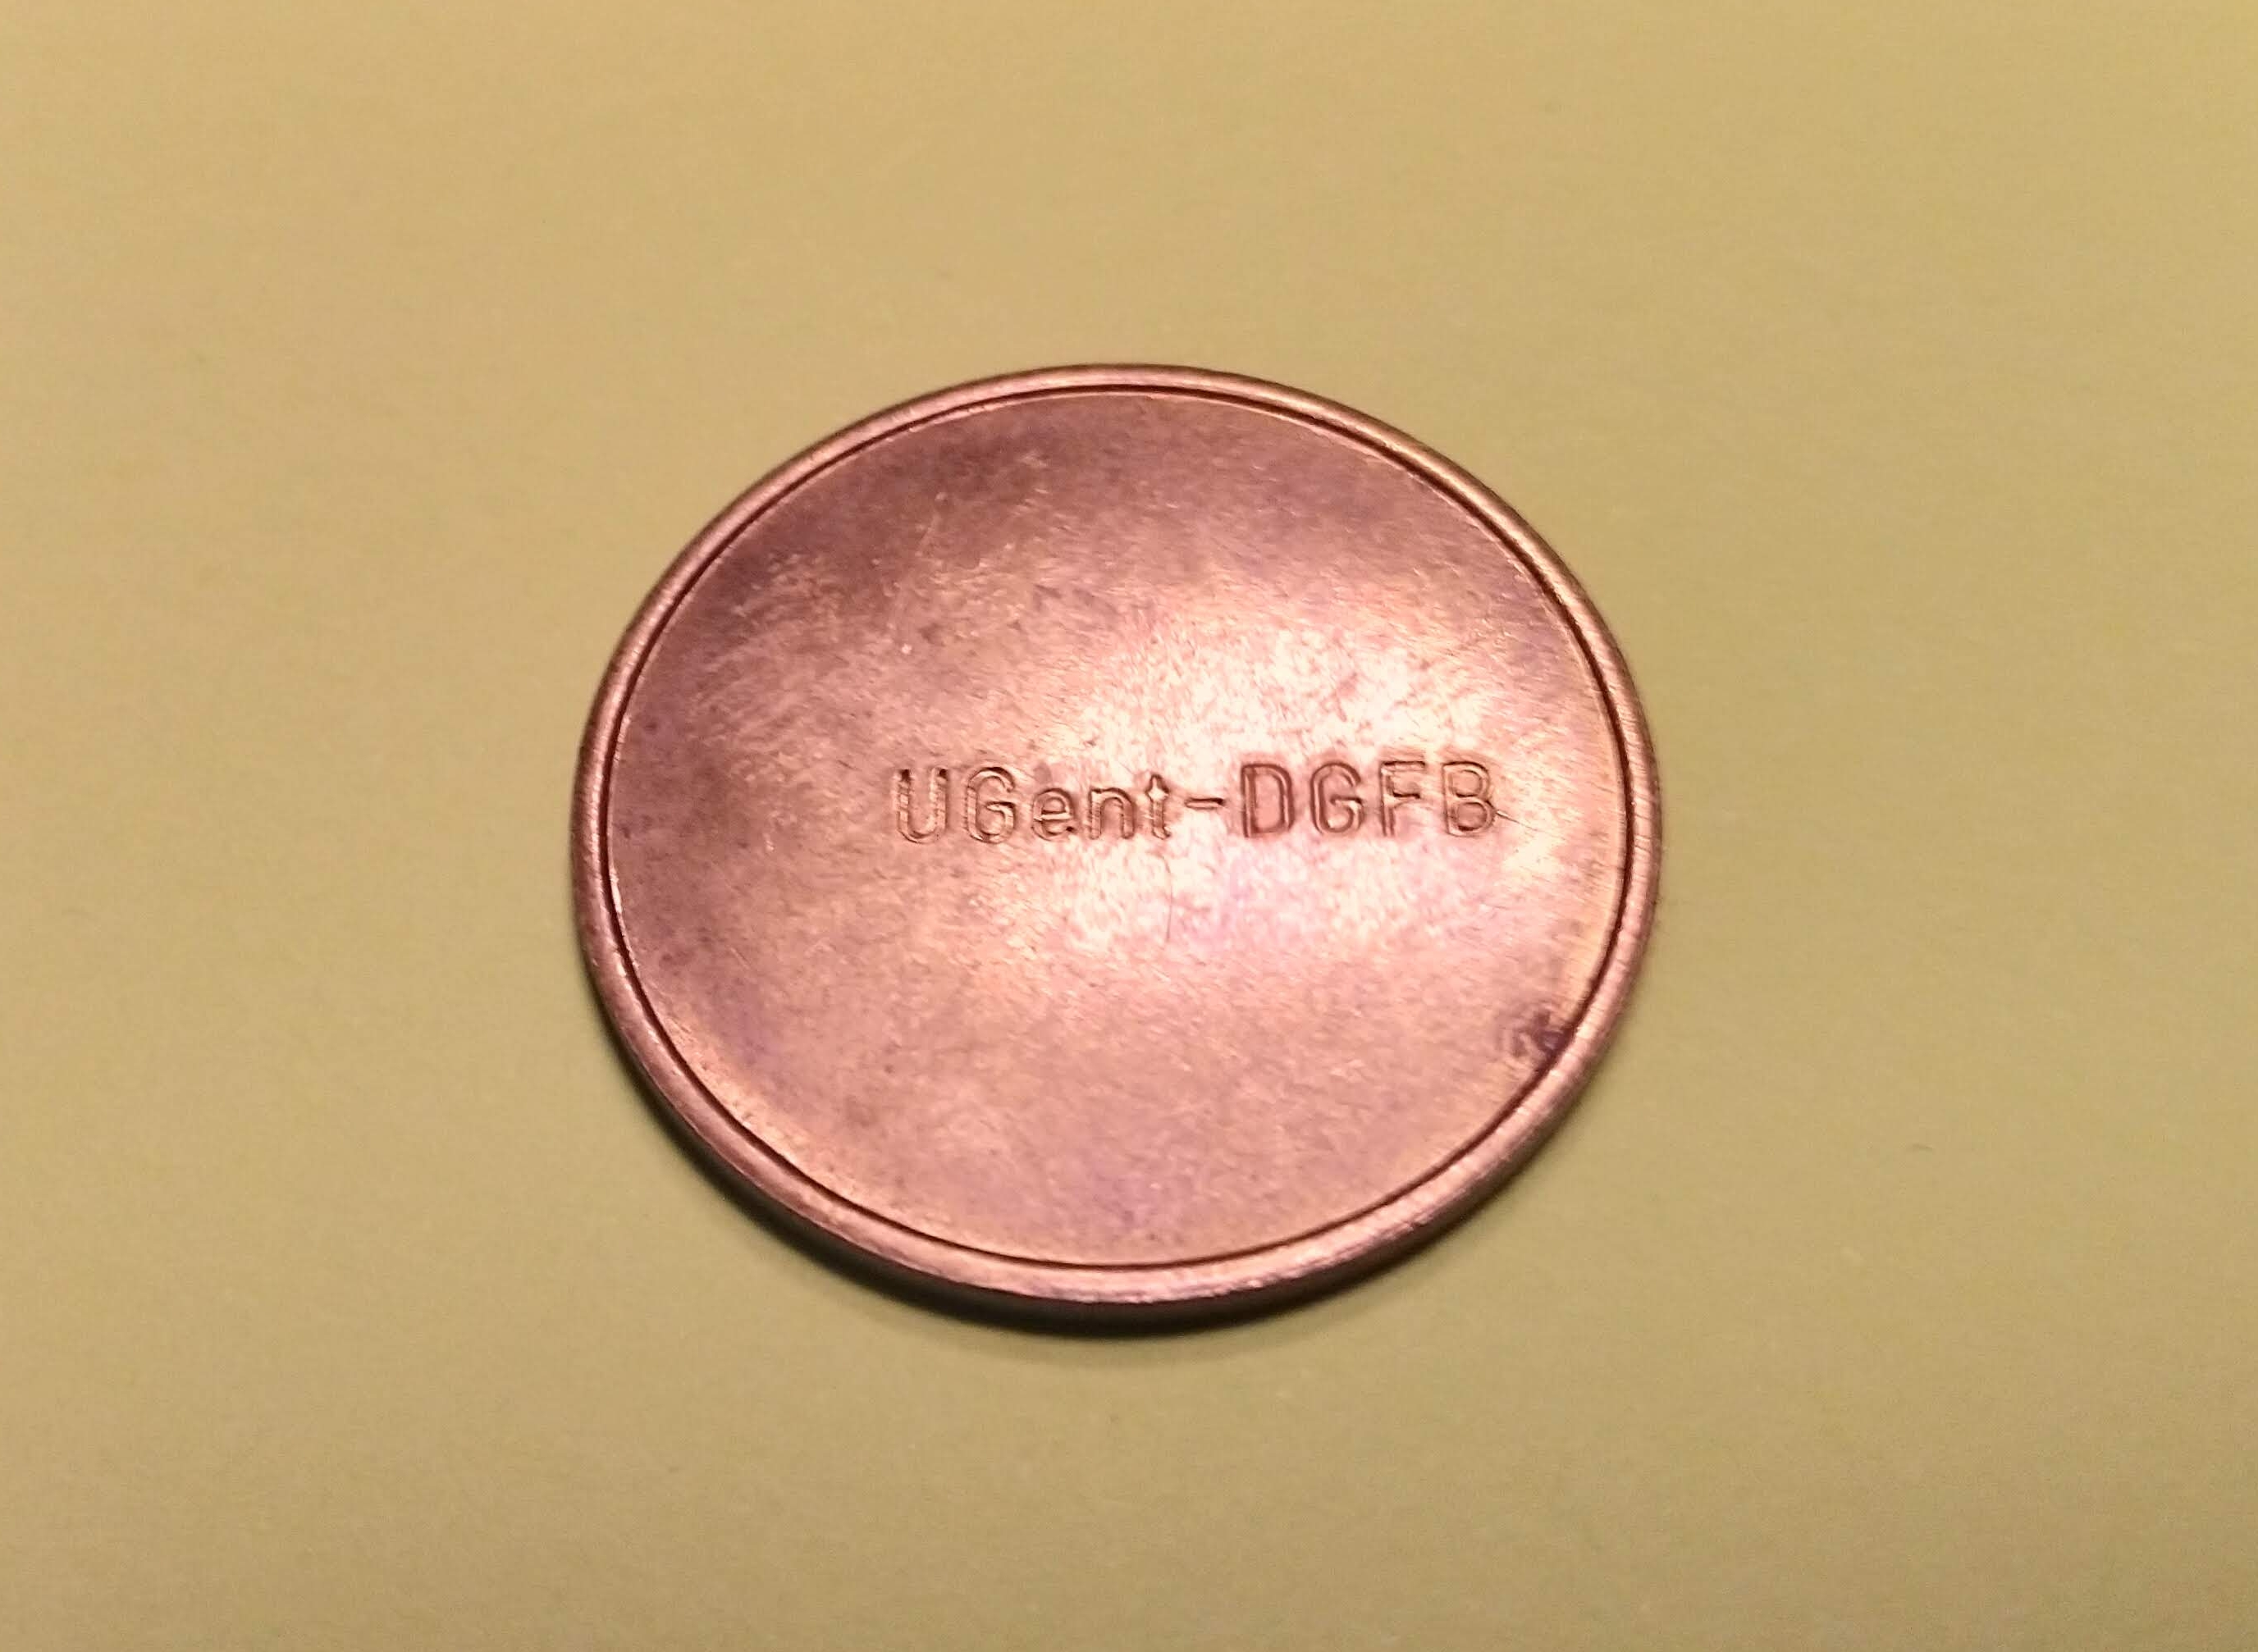
\includegraphics[width=0.5\linewidth]{img/token.jpg}
	\caption{Een huidige toegangstoken voor de parking van UGent te kunnen verlaten.}
\end{figure}

\subsubsection{Radio frequency Identification}

%Wat is RFID
Radio frequency Identication (RFID) is een technologie die aan de hand van elektromagnetische golven objecten kan identificeren. Dit met het voordeel dat er geen direct contact of zicht moet zijn tussen de scanner en het object. RFID gebeurt a.d.h.v een RFID reader en een RFID tag. De reader zendt een elektromagnetisch signaal uit. De tag ontvangt deze golven en kan op zijn beurt de opgevraagde informatie verzenden. \autocite{li2009design}

%RFID op UGent
Aan iedere uitgang op UGent zijn RFID-kaartlezers te vinden. Deze zijn voorzien om een vlotte toegang te verlenen aan werknemers en worden via een centraal beheerd systeem.

Het is geen optie om rfid voor alle bezoekers te gebruiken aangezien er vaak bezoekers binnentreden die maar 1 dag op de campus zijn. In dat geval zou er voor iedere dagbezoeker een RFID-kaart moet gemaakt worden. Aangezien de prijs van een RFID-kaart over de 10 euro is, is het zeker geen optie om dit als oplossing te gebruiken.

\subsubsection{Barcodes}
In een poging tot de tokens te vervangen heeft UGent één uitgang op de parking UFO en het rectoraat waar barcodes worden gebruikt. Deze worden eerst geprint op de campus zelf, waarna de gebruiker de barcode in een slikker kan invoeren en toegang krijgen om de parking te verlaten.

Deze barcodes hebben het grote voordeel dat ze goedkoper zijn in het gebruik. Maar hebben ze nog steeds het probleem dat iedere gebruiker telkens aan het onthaal een nieuw ticket moeten opvragen, en dat er slikkers slikkers aanwezig moeten zijn die tijdelijk geleegd worden.

Volgende lijst dient als een verduidelijking van de nadelen:
\begin{itemize}
	\item Milieubelasting, verspilling van papier
	\item ofwel moet een papierslikker geledigd worden ofwel zal er vervuiling zijn van achtergelaten papier aan de uitgang.
	\item Op diverse plaatsen moeten er drukkers aanwezig zijn.
\end{itemize}


\subsection{Mogelijkheid van ANPR}
De vorige technologieën zijn weliswaar niet de enige mogelijke oplossing tot dit probleem.

Automatic Number Plate Recognition (ANPR) is de techniek om automatisch nummerplaten te herkennen. Deze techniek wordt al sinds 1976 gebruikt voor voor de detectie van gestolen wagens \autocite{uk2011anpr}. Hedendaags is ANPR al veel toegankelijker en kan het op vele plaatsen teruggevonden worden zoals bij bv. trajectcontrole \autocite{de2014snelheidscamera}, parkeersystemen, etc.
\par
ANPR heeft nog vele andere acroniemen zoals Automatic License Plate Recognition (ALPR), Automatic Vehicle Identification (AVI), Vehicle Plate recognition (VLPR), Vehicle Recognition Identifier (VRI), Car plate Recognition (CPR) en Car Plate Reader (CPR) \autocite{axis2019license}. In dit onderzoek zal voor nummerplaatdetectie het acroniem ANPR gebruikt worden.
\par
%Voordelen
Het gebruik van ANPR brengt enkele voordelen met zich mee:
\begin{itemize}
	\item Het is heel modulair; mensen kunnen een dagpas of toegang voor een volledig schooljaar krijgen.
	\item Er moet slechts éénmalig aangemeld worden om toegang voor een langere periode te krijgen. Dit zou helemaal digitaal gedaan kunnen worden, wat personeelskosten bespaart.
	\item Indien succesvol geïmplementeerd kan ANPR opstoppingen aan toegangspunten verminderen omdat er geen menselijke interactie met het systeem meer nodig is.
\end{itemize}
\par
%Nadelen
ANPR zelf komt ook met enkele nadelen.
\begin{itemize}
	\item Er is een centraal systeem nodig om de toegang van de nummerplaten te beheren.
	\item Ieder toegangspunt moet een internetvoorziening hebben om met het centrale systeem te communiceren.
	\item Iedere ANPR-camera moet correct ingesteld zijn om haalbare resultaten te behalen.
	\item Weersomstandigheden bieden extra moeilijkheid voor de detectie van nummerplaten (dag, nacht)
	\item Hedendaagse ANPR-camera's zijn een redelijke investering.
\end{itemize}
\par
Voor de herkenning van nummerplaten zijn een aantal technologieën beschikbaar. Deze werken adhv. Artificial Intelligence (AI) en zijn specifiek getraind op het detecteren en uitlezen van nummerplaten.
De technologie die in dit onderwerp gebruikt zal worden is OpenALPR, een Open-Source library gemaakt voor nummerplaatdetectie. Hiervoor is gekozen omdat OpenALPR een gratis Open-Source product is \autocite{openalprgithub}.
%Nadelen


\section{Privacy en GDPR}
\label{sec:privacy-en-gdpr}

Sinds 25 Mei 2018 is de General Data Protection Regulation (GDPR) in gang gezet, een regulatie die ingevoerd is om het huidige  en toekomstige digitale tijdperk veiliger te maken voor alle EU inwoners.
Deze wetgeving is gedreven op het concept dat privacy een mensenrecht is, en dat online-data ook zo behandeld moet worden. Dit is data die direct of indirect gelinkt kan worden aan een individu zoals locatie-data, cookies en ip-adressen \autocite{goddard2017eu}.

Hierdoor komen er een groot aantal extra regels op bedrijven te liggen, zo zijn ze bvb. verplicht om te toestemming vragen om persoonsgegevens te mogen verwerken. Dit is merkbaar online, waar vele sites toestemming vragen om advertentie-cookies te mogen opslaan. Een heleboel andere regels zijn er ook bijgekomen, wat het moeilijk kan maken om een nieuw systeem te maken die aan al deze voldoet.

\section{Hardware}
Om deze nummerplaatdetectie uit te voeren is gekozen voor een Raspberry PI Model B+. Deze hardware wordt vandaag de dag veel gebruikt bij IOT-applicaties door zijn lage kost en gemakkelijke bruikbaarheid.  

De Raspberry PI Model B+ beschikt over een 1.4GHz quad-core processor, 1GB LPDDR2 RAM, een on-board WiFi-kaart en de mogelijkheid om een Raspberry Pi Camera te verbinden \autocite{raspberrypisitemodelbplus} .

\subsection{Camera}
De camera die gebruikt wordt is een Pi-NoIR camera. Deze camera is ook geproduceerd door de Raspberry Pi Foundation en biedt afbeeldingen en video in een 8-MegaPixel formaat. In dit onderzoek is voor deze camera gekozen omdat deze makkelijk te verbinden is met de Raspberry Pi, relatief goedkoop is en geen IR-filter heeft. Dit maakt de camera direct ook interessant voor foto's te nemen in donkere omgevingen. \autocite{raspberrypisitemodelpinoir}

\section{Software}
De software die gebruikt wordt in dit onderzoek is het open-source framework OpenALPR. Deze software is geschreven om nummerplaatdetectie uit te voeren en kan video's en foto's verwerken in een groot aanbod van programmeertalen \autocite{openalprgithub}. De keuze voor deze software is gemaakt door Vado-Solutions omdat OpenALPR open-source is, wat kosten dekt. Verder kan deze software ook gebruikt worden op Linux, wat noodzakelijk is om dit onderzoek uit te voeren met een Raspberry Pi.
%%=============================================================================
%% Methodologie
%%=============================================================================

\chapter{Methodologie}
\label{ch:methodologie}

%% TODO: Hoe ben je te werk gegaan? Verdeel je onderzoek in grote fasen, en
%% licht in elke fase toe welke stappen je gevolgd hebt. Verantwoord waarom je
%% op deze manier te werk gegaan bent. Je moet kunnen aantonen dat je de best
%% mogelijke manier toegepast hebt om een antwoord te vinden op de
%% onderzoeksvraag.

\lipsum[21-25]



% Voeg hier je eigen hoofdstukken toe die de ``corpus'' van je bachelorproef
% vormen. De structuur en titels hangen af van je eigen onderzoek. Je kan bv.
% elke fase in je onderzoek in een apart hoofdstuk bespreken.

%\input{...}
%\input{...}
%...

%%=============================================================================
%% Conclusie
%%=============================================================================

\chapter{Conclusie}
\label{ch:conclusie}

%% TODO: Trek een duidelijke conclusie, in de vorm van een antwoord op de
%% onderzoeksvra(a)g(en). Wat was jouw bijdrage aan het onderzoeksdomein en
%% hoe biedt dit meerwaarde aan het vakgebied/doelgroep? Reflecteer kritisch
%% over het resultaat. Had je deze uitkomst verwacht? Zijn er zaken die nog
%% niet duidelijk zijn? Heeft het onderzoek geleid tot nieuwe vragen die
%% uitnodigen tot verder onderzoek?

\lipsum[76-80]



%%=============================================================================
%% Bijlagen
%%=============================================================================

\appendix

%%---------- Onderzoeksvoorstel -----------------------------------------------

\chapter{Onderzoeksvoorstel}

Het onderwerp van deze bachelorproef is gebaseerd op een onderzoeksvoorstel dat vooraf werd beoordeeld door de promotor. Dat voorstel is opgenomen in deze bijlage.

% Verwijzing naar het bestand met de inhoud van het onderzoeksvoorstel
%---------- Inleiding ---------------------------------------------------------

\section{Introductie} % The \section*{} command stops section numbering
\label{sec:introductie}

Parkings zijn van groot belang in het dagelijks leven. Iedere dag rijden talloze wagens naar hun plaats om daar na een achttal uren weer opgepikt te worden. Ieder van deze wagens moet zich dan ook telkens identificeren om deze te betreden of te verlaten. Dit doen ze met behulp van tickets, badges of andere toegangssystemen. Ieder systeem heeft zijn eigen voor- en nadelen.

Dit onderzoek wordt uitgevoerd met oog op de parking van UGent, waar men kampt met enkele problemen met de toegang van de parking aan de Campus Sterre en Campus Coupure. Momenteel worden er op deze parkings tokens en badges gebruikt om de parking te verlaten, welke enkele negatieve punten met zich meebrengen. Zo worden de tokens snel kwijtgeraakt en zijn deze duur om bij te maken. Deze tokens zijn ook universeel en kunnen gebruikt worden bij andere diensten die soortgelijke tokens gebruiken. Verder moeten deze slikkers regelmatig geleegd worden, wat dan weer een personeelskost met zich meebrengt. Men heeft al enkele oplossingen bekeken om dit systeem te vervangen en een grote favoriet is het gebruik van nummerplaatdetectie waarbij met een centraal systeem specifieke wagens toegang kunnen krijgen.
\\
Vele manieren van toegangscontrole zijn allicht mogelijk en niets is perfect. In dit onderzoek wordt gekeken naar welke toegangstechnieken haalbaar zijn en welke voordelen deze leveren. Ook zal met oog op de voorkeur van UGent dieper ingegaan worden op nummerplaatdetectie. Hierbij zal er gekeken worden hoe dit opgeleverd kan worden waarbij de General Data Protection Regulation (GDPR) nageleefd wordt en of dit haalbaar is om uit te voeren op lichte hardware zoals een Raspberry PI.

Zo bekomen we volgende onderzoeksvragen:
\begin{itemize}
	\item Welke toegangstechnieken brengen het meest profijt voor de parking van UGent?
	\item Is nummerplaatdetectie een haalbare techniek omtrent privacy en GDPR?
	\item Kan men nummerplaatdetectie uitvoeren op een Raspberry PI?
\end{itemize}

%---------- Stand van zaken ---------------------------------------------------

\section{State-of-the-art}
\label{sec:state-of-the-art}

% UGent hedendaags met tokens
Vandaag de dag kampt UGent met verscheidene problemen met hun huidige toegangssysteem. Hierbij kunnen gebruikers de parking vrij binnenrijden, maar om deze te verlaten moeten ze een token verschaffen aan de campus zelf. Deze token moet vervolgens ingeworpen worden in de tokenslikker aan de uitgang, waarna de gebruiker de parking kan verlaten. Deze tokens hebben weliswaar enkele nadelen. Zo worden deze snel kwijtgeraakt en moeten deze bijgemaakt worden, wat een redelijke kost is en niet milieubewust is. Ook zijn deze tokens universeel en kunnen in eender welke tokenslikker ingevoerd worden.
% Uitgang Campus Coupure met tickets
\subsection{Papieren tickets}
Door de problemen die bij het gebruik van tokens te kijk komen heeft men op Campus Sterre intussen één uitgang waar gebruikt gemaakt wordt van papieren tickets. Dit was bedoeld als alternatief voor de tokens, maar aangezien deze papieren tickets gelijkaardige problemen met zich meebrengen zou dit geen gewenste oplossing brengen.
% RFID scanners op UGent
\subsection{RFID}
Verder heeft iedere uitgang ook een RFID-scanner die gebruikt wordt om toegang te verlenen aan personeel. RFID kan m.b.v. een centraal systeem personeelskosten verminderen \autocite{pala2007smart}, maar op een campus waar men soms bezoekers voor maar één dag heeft is het niet wenselijk om hiervoor badges te bedelen.
% Mogelijkheid van nummerplaatdetectie
\subsection{Nummerplaatdetectie}
Een andere, nog niet geïmplementeerde techniek is nummerplaatdetectie. Deze techniek veroorzaakt geen directe milieubelasting aangezien er geen tickets of badges worden gebruikt, maar waar deze techniek wel onder lijdt is de zichtbaarheid van de nummerplaten in slechte weersomstandigheden \autocite{azam2016automatic}. Hierbij moet dus onderzocht worden in welke mate dit haalbaar is in deze case.
\\
Dit onderzoek zal nagaan welke toegangstechnieken het voordeligst zijn en welke het beste is in de case van UGent. Dit gebeurt a.d.h.v. een vergelijkende studie op vlak van benodigde werkuren, milieubelastbaarheid, transparantie voor opvolging en toegangscontrole. Verder zal er uitgebreid gekeken worden hoe nummerplaatdetectie gebruikt kan worden zodat deze niet in strijd zijn met wetgevingen zoals de privacywetgeving en de GDPR. Ten slotte zal er gekeken worden of dit uitgevoerd kan worden op een kleine microcontroller zoals de Raspberry pi 3 B+ en of deze kwalitatieve resultaten biedt.

% Voor literatuurverwijzingen zijn er twee belangrijke commando's:
% \autocite{KEY} => (Auteur, jaartal) Gebruik dit als de naam van de auteur
%   geen onderdeel is van de zin.
% \textcite{KEY} => Auteur (jaartal)  Gebruik dit als de auteursnaam wel een
%   functie heeft in de zin (bv. ``Uit onderzoek door Doll & Hill (1954) bleek
%   ...'')

%---------- Methodologie ------------------------------------------------------
\section{Methodologie}
\label{sec:methodologie}

Vooraleer de onderzoeksvragen beantwoord worden is er nood aan inzicht in verschillende mogelijke toegangstechnieken voor parkings. Dit zal gedaan worden a.d.h.v. een literatuurstudie, waarbij dan ook de eerste onderzoeksvraag zal beantwoord worden. In deze literatuurstudie zullen de karakteristieken op vlak van milieuvriendelijkheid, gebruiksvriendelijkheid en kost vergeleken worden. Vervolgens zal hieruit de keuze gemaakt worden welke techniek het beste is voor een parking met meerdere toegangspunten.

Om de tweede onderzoeksvraag te kunnen beantwoorden zal nog een literatuurstudie uitgevoerd worden omtrent privacy en GDPR. Het doel hiervan is om richtlijnen te bekomen voor het gebruik van camera’s op een parking zonder wetgevingen te overtreden.

Voor de laatste onderzoeksvraag zal onderzocht worden of nummerplaatdetectie een haalbare technologie is om te gebruiken op een Raspberry Pi 3B+. Dit zal getest worden door foto’s te nemen van voertuigen aan de toegangspunten aan UGent, waarna er gekeken wordt of deze nummerplaten detecteerbaar zijn met de Raspberry Pi. En of dit in een realistische tijd uitgevoerd kan worden met een acceptabele foutratio.

%---------- Verwachte resultaten ----------------------------------------------
\section{Verwachte resultaten}
\label{sec:verwachte_resultaten}

Er wordt verwacht dat nummerplaatdetectie het meest profijtelijk zal zijn in het geval van de parking van de UGent door de lagere kosten. Aan de toegangspunten zouden enkel camera’s en microcontrollers geïnstalleerd moeten worden, wat met de huidige netwerkinfrastructuur geen probleem moet zijn. Het implementeren van andere technieken zoals tickets zou ook een verbetering zijn, maar is nadeliger voor het milieu en brengt meer personeelswerk met zich mee zoals het legen van de slikkers en het aanvullen van de tickets. Voor nummerplaatdetectie foutmarge wordt verwacht dat 5\% van de inlezingen foutief zijn. Deze marge wordt genomen uit het onderzoek van \textcite{figuerola2016automated} waar men in optimale omstandigheden 94.4\% nauwkeurigheid gehaald heeft met gelijkaardige technologieen.

%---------- Verwachte conclusies ----------------------------------------------
\section{Verwachte conclusies}
\label{sec:verwachte_conclusies}

Indien de testresultaten van de nummerplaatdetectie hoog genoeg zijn en deze duidelijke voordelen heeft tegenover andere technieken, mogen we concluderen dat dit een haalbare toegangstechniek is voor de parking bij de UGent.


%%---------- Andere bijlagen --------------------------------------------------
% TODO: Voeg hier eventuele andere bijlagen toe
%\input{...}

%%---------- Referentielijst --------------------------------------------------

\printbibliography[heading=bibintoc]
%\addcontentsline{toc}{chapter}{\textcolor{maincolor}{\IfLanguageName{dutch}{Bibliografie}{Bibliography}}}

\end{document}
